\documentclass[11pt]{article}


\usepackage{tkz-euclide}
%\usepackage{tkz-base}
%\usetikzlibrary{calc,patterns,angles,quotes,babel}
\usepackage{tkz-euclide}
\usepackage{pgfplots}
\usetkzobj{all}
\usetikzlibrary{shapes.geometric}
\usepackage{amssymb}

\usepgflibrary{arrows}
\usetikzlibrary{arrows} 
\pgfplotsset{compat=newest}
\begin{document}
\section{Module 1: Elementaire rekenvaardigheden A}
%\input{1_elem_rekenvaardigheden_A/inputs/absvalue}
%\input{dimitri_oefent_tikz}
%\input{1_elem_rekenvaardigheden_A/inputs/absvalue_2}
%\input{1_elem_rekenvaardigheden_A/inputs/logFunc1}

%\input{1_elem_rekenvaardigheden_A/inputs/logFunc2}
\section{Module 2: Elementaire rekenvaardigheden B}
\subsection{re\"ele functie vb1}
\begin{center}	
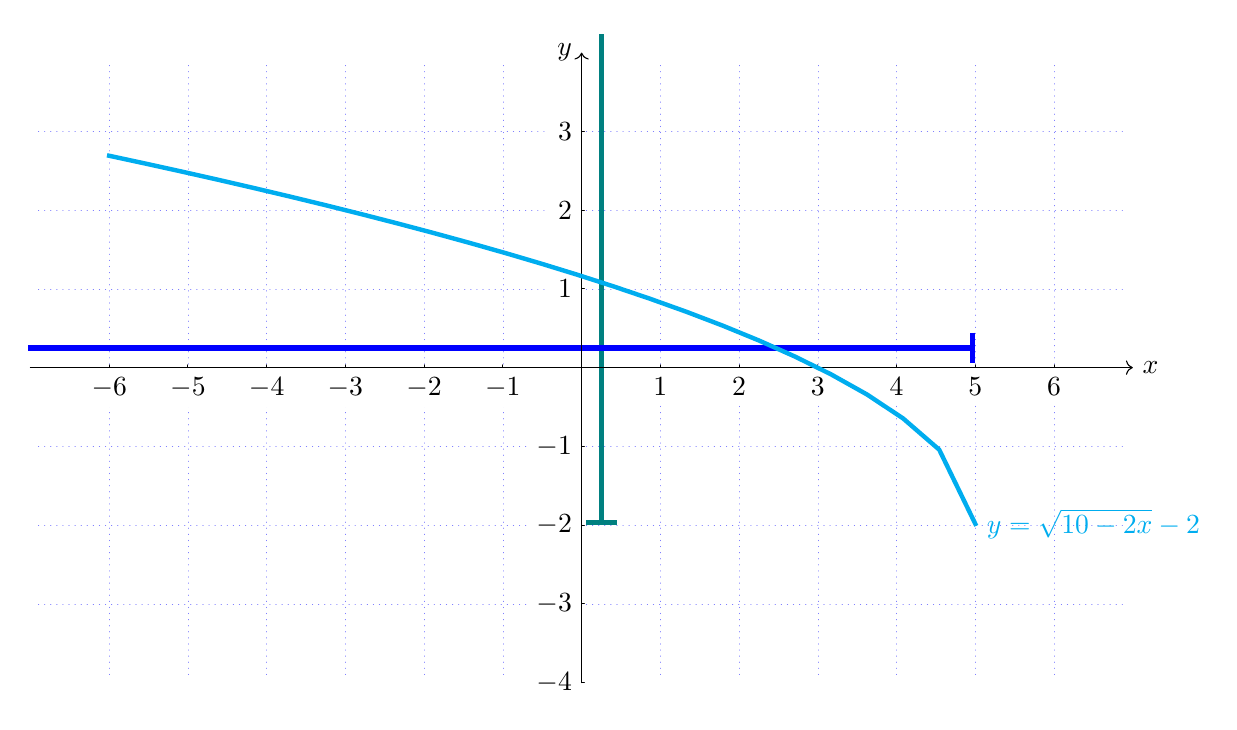
\begin{tikzpicture}[scale=1,cap=round]

% Styles
\tikzstyle{axes}=[]
\tikzstyle help lines=[color=blue!50,very thin,dotted]


%%%%%%%%%%%%%%%%%%%%%%%%%%%%%%%%
%		GRID
%%%%%%%%%%%%%%%%%%%%%%%%%%%%%%%%

\draw[style=help lines,step=1cm] (-6.9,-3.9) grid (6.9,3.9);


%%%%%%%%%%%%%%%%%%%%%%%%%%%%%%%%
%		MARKERINGEN
%%%%%%%%%%%%%%%%%%%%%%%%%%%%%%%%
\draw[ |-,line width=2,teal, cap=rect,] (0.25,-2) -- (0.25,4.2) node[right] {};
\draw[arrows=-|,line width=2,blue, cap=rect,] (-7,0.25) -- (5,0.25) node[right] {};


%%%%%%%%%%%%%%%%%%%%%%%%%%%%%%%%
%		ASSENSTELSEL
%%%%%%%%%%%%%%%%%%%%%%%%%%%%%%%%

\draw[->] (-7,0) -- (7,0) node[right] {$x$};
\draw[->] (0,-4) -- (0,4) node[left]{$y$};

%\draw[fill,cyan](1,1)circle [radius=0.025];

%\draw[red,cap=rect, loosely dashed, ultra thick, domain=-2:2] plot (\x, {(\x*\x-1)+0.05}) node[above,yshift=-.7cm, right]{};

%%%%%%%%%%%%%%%%%%%%%%%%%%%%%%%%
%legende
%%%%%%%%%%%%%%%%%%%%%%%%%%%%%%%%
%\tkzDefPoint(0.5,3.5){A}
%\tkzDefPoint(1,3.5){B}
%\tkzLabelPoint[right,xshift=+0.1cm](B){${\color{cyan}f(x)=|x^2-1|}$}
%\tkzDrawSegment[cyan,ultra thick](A,B)

%\tkzDefPoint(0.5,3.2){C}
%\tkzDefPoint(1,3.2){D}
%\tkzLabelPoint[right,xshift=+0.1cm](D){${\color{red}e(x)=x^2-1}$}
%\tkzDrawSegment[red,cap=rect, loosely dashed, ultra thick](C,D)


%%%%%%%%%%%%%%%%%%%%%%%%%%%%%%%%
%getallen op de x-as en lijntjes
%%%%%%%%%%%%%%%%%%%%%%%%%%%%%%%%   
\foreach \x/\xtext in {-6,-5,-4,-3,-2,-1,1,2,3,4,5,6}
	\draw[xshift=\x cm] (0pt,1pt) -- (0pt,0pt) node[below,fill=white]
	{$\xtext$};,3
	
%getallen op de y-as en lijntjes  
%BEGIN LUS
\foreach \y/\ytext in {-4,-3,-2,-1,1,2,3}
	\draw[yshift=\y cm] (1pt,0pt) -- (0pt,0pt) node[left,fill=white]
	{$\ytext$}; %EINDE LUS



%%%%%%%%%%%%%%%%%%%%%%%%%%%%%%%%
%		GRAFIEKEN
%%%%%%%%%%%%%%%%%%%%%%%%%%%%%%%%
%\draw[cyan,cap=rect,thick, domain=-6:6] plot (\x, \x) node[above, right]{${\color{cyan}y=x}$};v

\draw[cyan,cap=rect,ultra thick, domain=-6:5] plot (\x, {sqrt(10-2*\x)-2}) node[above, right]{${\color{cyan}y=\sqrt{10-2x}-2}$};



%\draw[cyan,cap=rect,ultra thick, domain=-7:1.9] plot (\x, {exp{\x}}) node[above, right]{${\color{cyan}y=\exp{x}}$};


\end{tikzpicture}
\end{center}
\newpage
\input{2_elem_rekenvaardigheden_B/inputs/reele_functies_vb2}
\input{2_elem_rekenvaardigheden_B/inputs/reele_functies_vb3}
\input{2_elem_rekenvaardigheden_B/inputs/verloop_vb1}
\input{2_elem_rekenvaardigheden_B/inputs/verloop_vb2}
\input{2_elem_rekenvaardigheden_B/inputs/verloop_vb3}
%TODO waarom verschijnt dat hier niet? 

%\begin{center}
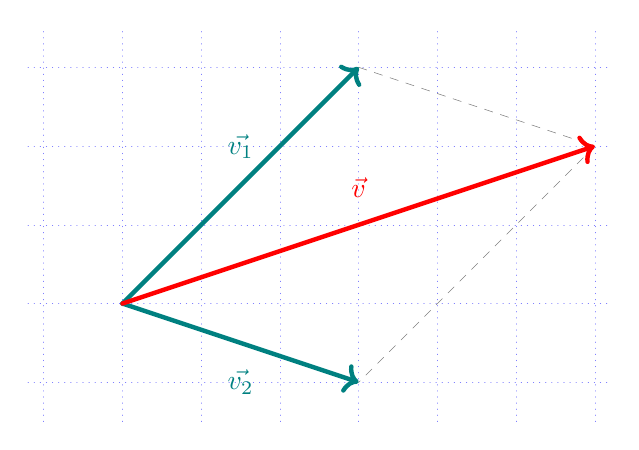
\begin{tikzpicture}[scale=1,cap=round]

% Styles
\tikzstyle{axes}=[]
\tikzstyle help lines=[color=blue!50,very thin,dotted]

% grid
\draw[style=help lines,step=1cm] (-1.2,-1.5) grid (6.2,3.5);



\tkzDefPoint(3,3){A}
\tkzDefPoint(6,2){B}
\tkzDefPoint(3,-1){C}
%\tkzDefPoint(1,1){D}
%\tkzDefPoint(2,2){E}
\tkzDrawSegment[gray,dashed,cap=rect](A,B)
\tkzDrawSegment[gray,dashed,cap=rect](B,C)


\draw[->,teal,ultra thick] (0,0) -- (3,3) node[pos=0.5,above,yshift=+0.2cm] {${\Huge\vec{v_1}}$};
\draw[->,teal,ultra thick] (0,0) -- (3,-1) node[pos=0.5,below,yshift=-0.2cm] {$\vec{v_2}$};
\draw[->,red,ultra thick] (0,0) -- (6,2) node[pos=0.5,above,yshift=+0.2cm] {$\vec{v}$};


\end{tikzpicture}
\end{center}
\newpage
%\input{1_elem_rekenvaardigheden_A/inputs/kopstaart}

\end{document}